Let us now use Euler's explicit method to solve the equation $\dfrac{dU}{d \tau}= AU+b(\tau)$ in time. The scheme gives
\begin{align*}
U^{k+1} &= U^{k} + \Delta t\Big(\dfrac{1}{h^2}AU^{k}+\dfrac{1}{h^2}b(\tau)\Big)\\
 &= \Big( I_{N} + \dfrac{\Delta t}{h^2} A\Big)U^{k} + \dfrac{\Delta t}{h^2}\cdot b(\tau)
\end{align*}
The code is available below in \ttt{tempEE.m}.

We present a stable and an unstable solution on the figures~\ref{fig:stable}\ref{fig:unstable}.
They were obtained respectively with the calls \ttt{tempEE(10,0.005,2)} and \ttt{tempEE(10,0.0051,2)}. This corresponds to $\Delta x = 0.1$ and $\Delta t = \{0.005, 0.0051 \}$. This gives $\dfrac{\Delta t}{\Delta x^2}= \{0.5,0.51\}$. The unstable case breaks the condition $\dfrac{\Delta t}{\Delta x^2}\leq \dfrac{1}{2}$.


\begin{figure}[!h]
\centering
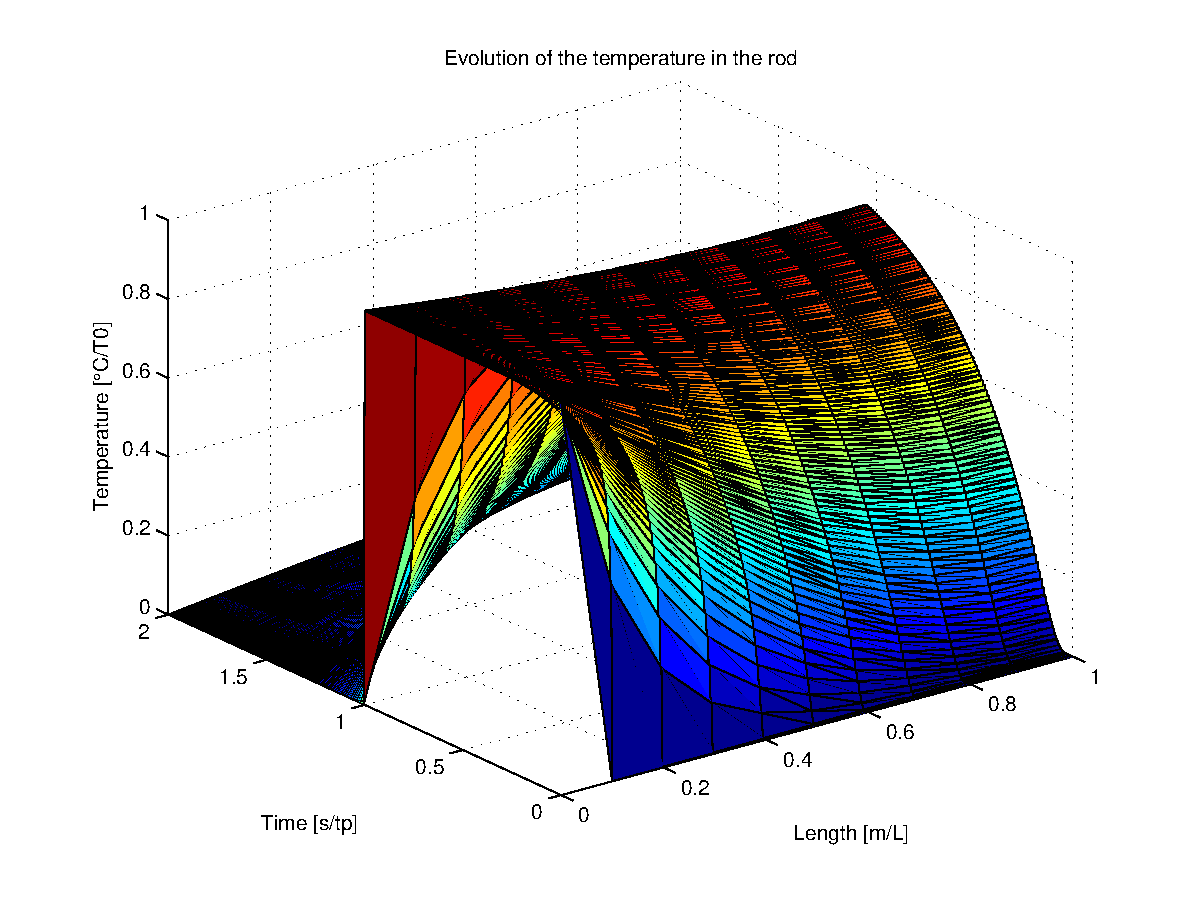
\includegraphics[width = 0.7\textwidth]{./stable.eps}
\caption{Stable solution: }
\label{fig:stable}
\end{figure}

\begin{figure}[!h]
\centering
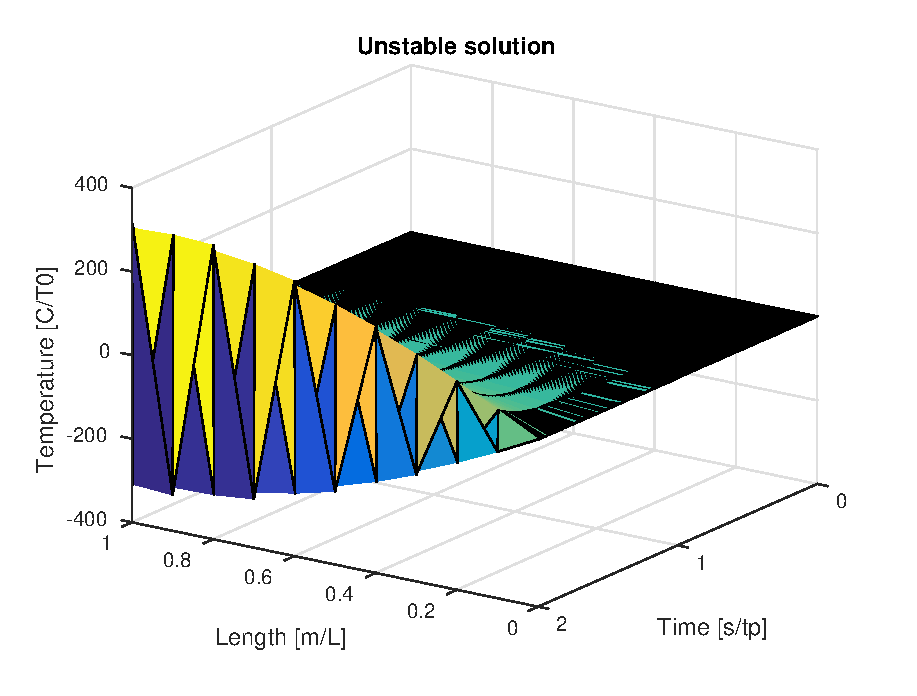
\includegraphics[width = 0.7\textwidth]{./unstable.eps}
\caption{Unstable solution: }
\label{fig:unstable}
\end{figure}
\FloatBarrier
